% Generated by pipeline/paper/scripts/make_result_figures.py. Do not edit by hand.
% R3c primary partition. Rows consistent with each scored normalizer.
% Shared figure style. Input once; a second input is a no-op.
\ifdefined\actsplotsready
\else
  \def\actsplotsready{1}
  \colorlet{actsteal}{teal!72!black}
  \colorlet{actstealfaint}{teal!16}
  \colorlet{actsorange}{orange!88!black}
  \colorlet{actsink}{black!80}
  \colorlet{actsghost}{black!45}
  \colorlet{actsfail}{red!62!black}
  \colorlet{actsrule}{black!50}
  \usetikzlibrary{intersections}
  \usepgfplotslibrary{fillbetween,groupplots}
  \pgfplotsset{
    acts/.style={
      font=\scriptsize\sffamily,
      tick label style={font=\scriptsize\sffamily},
      label style={font=\scriptsize\sffamily},
      legend style={
        font=\scriptsize\sffamily,
        draw=none,
        fill=none,
        cells={anchor=west},
        inner sep=1pt,
        column sep=6pt
      },
      legend cell align=left,
      scale only axis,
      clip=false,
      axis line style={actsrule},
      tick style={actsrule},
      tick align=outside,
      axis lines=left,
      xmajorgrids=true,
      major grid style={black!7},
      ymajorgrids=false,
      every node/.append style={font=\scriptsize\sffamily, inner sep=1.5pt},
      every axis plot/.append style={line join=round, line cap=round},
    },
  }
  \tikzset{
    actlab/.style={
      font=\scriptsize\sffamily,
      fill=white,
      fill opacity=0.92,
      text opacity=1,
      inner sep=1.35pt,
      outer sep=0.5pt,
    },
  }
\fi

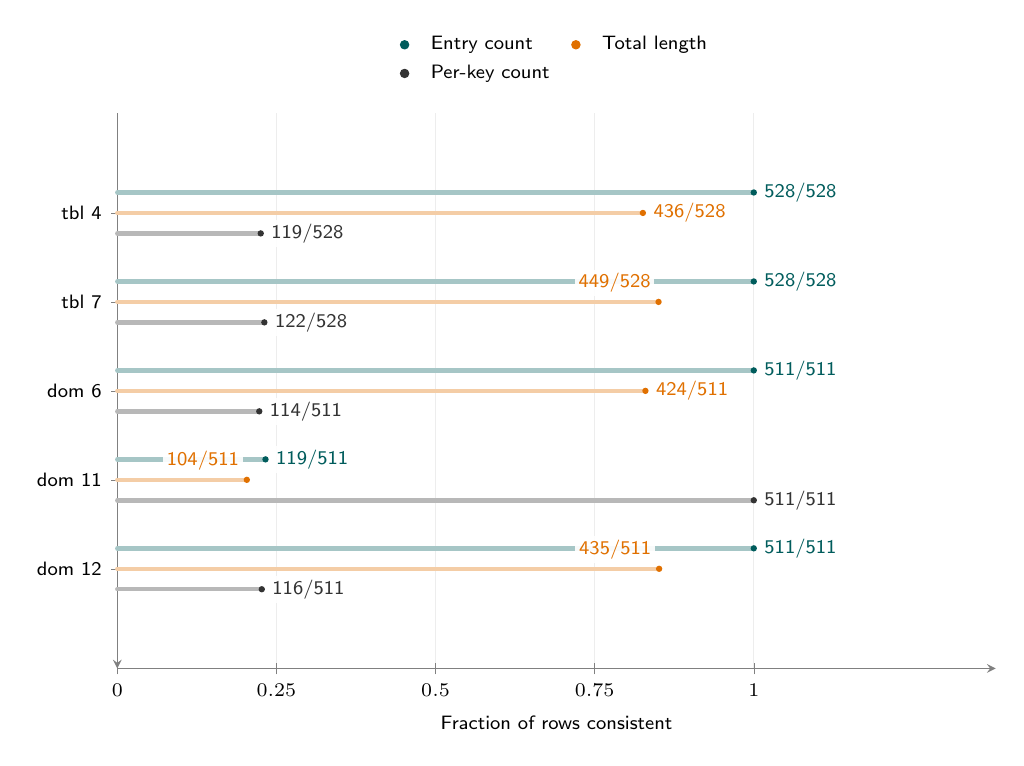
\begin{tikzpicture}
\begin{axis}[
  acts,
  width=0.92\columnwidth,
  height=7.05cm,
  xmin=0, xmax=1.38,
  xtick={0,0.25,0.5,0.75,1},
  xlabel={Fraction of rows consistent},
  ytick={0,...,4},
  yticklabels={{tbl 4},{tbl 7},{dom 6},{dom 11},{dom 12}},
  y dir=reverse,
  enlarge y limits=0.28,
  legend style={at={(0.5,1.04)}, anchor=south, legend columns=2},
]
\addplot[draw=none, forget plot] coordinates {(0,0) (1,4)};
\addlegendimage{only marks, mark=*, mark size=1.5pt, fill=actsteal, draw=actsteal}
\addlegendimage{only marks, mark=*, mark size=1.5pt, fill=actsorange, draw=actsorange}
\addlegendimage{only marks, mark=*, mark size=1.5pt, fill=actsink, draw=actsink}
\addlegendentry{Entry count}
\addlegendentry{Total length}
\addlegendentry{Per-key count}
% source: reference_fitter_t1.json r3c.primary_residuals entry_count
\draw[actsteal!35, line width=1.6pt, line cap=round] (axis cs:0,-0.2300) -- (axis cs:1,-0.2300);
\fill[actsteal] (axis cs:1,-0.2300) circle[radius=1.15pt];
\draw[actsteal!35, line width=1.6pt, line cap=round] (axis cs:0,0.7700) -- (axis cs:1,0.7700);
\fill[actsteal] (axis cs:1,0.7700) circle[radius=1.15pt];
\draw[actsteal!35, line width=1.6pt, line cap=round] (axis cs:0,1.7700) -- (axis cs:1,1.7700);
\fill[actsteal] (axis cs:1,1.7700) circle[radius=1.15pt];
\draw[actsteal!35, line width=1.6pt, line cap=round] (axis cs:0,2.7700) -- (axis cs:0.23287671,2.7700);
\fill[actsteal] (axis cs:0.23287671,2.7700) circle[radius=1.15pt];
\draw[actsteal!35, line width=1.6pt, line cap=round] (axis cs:0,3.7700) -- (axis cs:1,3.7700);
\fill[actsteal] (axis cs:1,3.7700) circle[radius=1.15pt];
% source: reference_fitter_t1.json r3c.primary_residuals total_entry_length
\draw[actsorange!35, line width=1.6pt, line cap=round] (axis cs:0,0.0000) -- (axis cs:0.82575758,0.0000);
\fill[actsorange] (axis cs:0.82575758,0.0000) circle[radius=1.15pt];
\draw[actsorange!35, line width=1.6pt, line cap=round] (axis cs:0,1.0000) -- (axis cs:0.85037879,1.0000);
\fill[actsorange] (axis cs:0.85037879,1.0000) circle[radius=1.15pt];
\draw[actsorange!35, line width=1.6pt, line cap=round] (axis cs:0,2.0000) -- (axis cs:0.8297456,2.0000);
\fill[actsorange] (axis cs:0.8297456,2.0000) circle[radius=1.15pt];
\draw[actsorange!35, line width=1.6pt, line cap=round] (axis cs:0,3.0000) -- (axis cs:0.2035225,3.0000);
\fill[actsorange] (axis cs:0.2035225,3.0000) circle[radius=1.15pt];
\draw[actsorange!35, line width=1.6pt, line cap=round] (axis cs:0,4.0000) -- (axis cs:0.85127202,4.0000);
\fill[actsorange] (axis cs:0.85127202,4.0000) circle[radius=1.15pt];
% source: reference_fitter_t1.json r3c.primary_residuals per_key_row_count:tblout
\draw[actsink!35, line width=1.6pt, line cap=round] (axis cs:0,0.2300) -- (axis cs:0.22537879,0.2300);
\fill[actsink] (axis cs:0.22537879,0.2300) circle[radius=1.15pt];
\draw[actsink!35, line width=1.6pt, line cap=round] (axis cs:0,1.2300) -- (axis cs:0.23106061,1.2300);
\fill[actsink] (axis cs:0.23106061,1.2300) circle[radius=1.15pt];
\draw[actsink!35, line width=1.6pt, line cap=round] (axis cs:0,2.2300) -- (axis cs:0.22309198,2.2300);
\fill[actsink] (axis cs:0.22309198,2.2300) circle[radius=1.15pt];
\draw[actsink!35, line width=1.6pt, line cap=round] (axis cs:0,3.2300) -- (axis cs:1,3.2300);
\fill[actsink] (axis cs:1,3.2300) circle[radius=1.15pt];
\draw[actsink!35, line width=1.6pt, line cap=round] (axis cs:0,4.2300) -- (axis cs:0.22700587,4.2300);
\fill[actsink] (axis cs:0.22700587,4.2300) circle[radius=1.15pt];
\node[actlab, anchor=west, text=actsink, xshift=2pt] at (axis cs:0.22537879,0.2300) {119/528};
\node[actlab, anchor=west, text=actsorange, xshift=2pt] at (axis cs:0.82575758,0.0000) {436/528};
\node[actlab, anchor=west, text=actsteal, xshift=2pt] at (axis cs:1,-0.2300) {528/528};
\node[actlab, anchor=west, text=actsink, xshift=2pt] at (axis cs:0.23106061,1.2300) {122/528};
\node[actlab, anchor=south east, text=actsorange, xshift=-1pt, yshift=1.5pt] at (axis cs:0.85037879,1.0000) {449/528};
\node[actlab, anchor=west, text=actsteal, xshift=2pt] at (axis cs:1,0.7700) {528/528};
\node[actlab, anchor=west, text=actsink, xshift=2pt] at (axis cs:0.22309198,2.2300) {114/511};
\node[actlab, anchor=west, text=actsorange, xshift=2pt] at (axis cs:0.8297456,2.0000) {424/511};
\node[actlab, anchor=west, text=actsteal, xshift=2pt] at (axis cs:1,1.7700) {511/511};
\node[actlab, anchor=south east, text=actsorange, xshift=-1pt, yshift=1.5pt] at (axis cs:0.2035225,3.0000) {104/511};
\node[actlab, anchor=west, text=actsteal, xshift=2pt] at (axis cs:0.23287671,2.7700) {119/511};
\node[actlab, anchor=west, text=actsink, xshift=2pt] at (axis cs:1,3.2300) {511/511};
\node[actlab, anchor=west, text=actsink, xshift=2pt] at (axis cs:0.22700587,4.2300) {116/511};
\node[actlab, anchor=south east, text=actsorange, xshift=-1pt, yshift=1.5pt] at (axis cs:0.85127202,4.0000) {435/511};
\node[actlab, anchor=west, text=actsteal, xshift=2pt] at (axis cs:1,3.7700) {511/511};
\end{axis}
\end{tikzpicture}
